
\chapter{Matchings}
Given the graph $G = (V, E)$, the set $M \subseteq E$ is a \textit{matching} if all edges in $M$ are independent. That is, no two edges share an endpoint. The size of a matching is the number of edges it contains.\\

For the graph $G$, $X \subseteq V$ is a \textit{vertex cover} if every edge in $E$ has at least one endpoint in $X$.\\

A \textit{perfect matching} (a.k.a. 1-factor) is a matching with $|M| = \frac{|V|}{2}$.
That is, every vertex of the graph is incident to exactly one edge of the matching. Every perfect matching is maximum and hence maximal. In some literature, the term complete matching is used. A perfect matching is also a minimum-size edge cover. \\

Observation: if $M$ is a matching and $X$ a vertex cover, then $|X| \geq |M|$. Corollary: the minimum size of a vertex cover is $\geq$ the maximum size of a matching.

\section{Matching in bipartite graphs}
For this whole section, we let $G = (V, E)$ be a fixed bipartite graph with bipartition $\{A, B \}$. Vertices denoted as $a, a'$, etc. will be assumed to lie in $A$, vertices noted as $b$ etc. will lie in $B$.\\

An \textit{alternating path} (w.r.t. some matching $M$) is a path in $G$ that starts at an unmatched vertex in $A$ and alternates between edges in $E-M$ and edges in $M$ (it can be made of only one edge).\\

An \textit{augmenting path} (w.r.t. some matching $M$) is an alternating path whose end will be at an unmatched vertex (of $B$). Note that if $P$ is an augmenting path, then $M \Delta E(P)$ \footnote{$\Delta$, a symmetric difference, defined as $X \Delta Y = (X-Y) \cup (Y-X) = (X \cup Y) - (X \cap Y)$} is again a matching, of size $|M| + 1$. \\

Alternating paths play an important role in the practical search for large matchings. In fact, if we start with any matching and keep applying augmenting paths until no further such improvement is possible, the matching obtained will always be an optimal one, a matching with the largest possible number of edges.

\subsection{König's theorem (1931)} 

\textit{The maximum cardinality of a matching in $G$ is equal to the minimum cardinality of a vertex cover.}\\

Let $G = (V,E)$ be a bipartite graph with bipartition $V = (A, B)$. Then the maximum size of a matching in $G$ is the minimum size of a vertex cover in $G$.
	\begin{enumerate}
		\item Let $M$ be a maximum matching. From every edge in $M$ let us choose one of its ends: its end in $B$ if some alternating path ends in that vertex, and its end in $A$ otherwise. We shall prove that this set of these $|M|$ vertices - let us name it $U$ - covers $E$; since any vertex cover of $E$ must cover $M$, there can be none with fewer than $|M|$ vertices, and so the theorem will follow.
		\item Let $ab \in E$ be an edge; we show that either $a$ or $b$ lies in $U$. If $ab \in M$, this holds by definition of $U$ - so we assume that $ab \notin M$. Since $M$ is a maximal matching, there is an edge $a'b' \in M$ with $a = a'$ or $b = b'$ For all $ab \notin M$, we have:
			\begin{enumerate} 
				\item First, let's assume $b = b'$: $a$ is the unmatched start of $ab$, which is then an alternating path, and so the end of $a'b' \in M$ chosen for $U$ was the vertex $b' = b$.
				\item Now with $a' = a$. If the start $a = a'$  is not in $U$, then $b' \in U$ (as $a'b'$ is an edge in $M$), and some alternating path $P$ ends in $b'$ (by definition of $U$). But then there is also an alternating path $P'$ ending in $b$, either $P := Pb$ (if $b \in P$) or $P' := Pb'a'b$. By the maximality of $M$, however, $P'$ can't be an augmenting path. So $b$ must be matched, and was chosen for $U$ from the edge of $M$ containing it.
			\end{enumerate}
	\end{enumerate}
	
\subsection{Hall's theorem (1935)} 

\textit{If $G$ is bipartite with partitions $A,B$, it contains a matching of $A$ if and only if $|N(S) \geq |S|$ for all $S \subseteq A$ (marriage condition).}\\

Here, $N(S) = \{ x \in B $ s.t. $x$ is adjacent to some vertex in $S \}$.\\

\begin{figure}[H]
	\center
	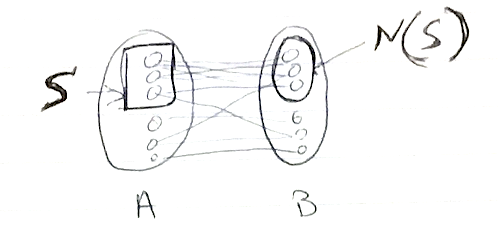
\includegraphics{img/2-1.png}
\end{figure}  
Let $G = (V, E)$ be a bipartite graph with bipartition $V = (A, B)$. Then (keeping in mind that for each partition $X$, any $x \in X$ isn't connected to any other $x' \in X$):
\begin{eqnarray}
	A \text{ can be matched } \iff |N(S)| \geq |S| ~~\forall S \subseteq A
\end{eqnarray} 
Proving both implications:
\begin{enumerate}
	\item $\implies$: done orally, quite intuitive.
	\item $\impliedby$: we prove the contrapositive\footnote{The contrapositive of a statement has its antecedent and consequent inverted and flipped: the contrapositive of $P \rightarrow Q$ is thus $\neg Q \rightarrow \neg P$}: if $A$ cannot be matched then $\exists S \subseteq A$ such that $|N(S) < |S|$. So assume $A$ cannot be matched:
		\begin{eqnarray}
			A \text{ can be matched } &\impliedby& |N(S)| \geq |S| ~~\forall S \subseteq A \\
		\end{eqnarray}
		is equivalent to:
		\begin{eqnarray}
			A \text{ cannot be matched } &\implies& \exists S \subseteq A : N(S) < |S|
		\end{eqnarray} 
	\item If $G$ contains no matching of $A$, then by König's theorem, it has a cover $U$ with fewer than $A$ vertices:
		\begin{eqnarray}
			|A \cap U| + |B \cap U| < |A|
		\end{eqnarray}
		hence:
		\begin{eqnarray}
			|B \cap U| < |A| - |A \cap U| = |A \setminus (A \cap U)|
		\end{eqnarray}
	\item By defintion of $U$, $G$ has no edge between $A \setminus (A \cap U)$ and $B \setminus (B \cap U)$. Let $A \setminus (A \cap U)$:
		\begin{eqnarray}
			|N(S)| \leq |B \cap U| < |A \setminus (A \cap U)| = |S|
		\end{eqnarray} 
		and the marriage condition fails.
\end{enumerate}

\bigskip
$\mu(G) := \mu := |\text{max matching}|$\\
$\tau(G) := \tau := |\text{min vertex cover}|$

$G$ bipartite $\Rightarrow \mu(G) = \tau(G)$\\
In general $\Rightarrow \mu(G) \leq \tau(G) \leq 2 \mu(G)$

\section{Matching in general graphs}
\textit{Component} (or \textit{connected component}) is a connected subgraph which is inclusion wise
maximal with this property.

Observation: every component of $G$ is an induced subgraph of $G$.

\bigskip
Given a graph $G$, let us denote by $\mathcal{C}_G$ the set of its components, and by $q(G)$ the number of its odd components, those of odd order.


		\subsection{Tutte's theorem (1947)} 
		
		\textit{A graph $G$ has a perfect matching if and only if $q(G - S) \leq |S|$ for all $S \subseteq V(G)$.}\\

                $\Rightarrow$)
                Obviously, every odd component of $G - S$ is linked to $S$ by at least one edge from the matching $M$ (because of parity). Hence $|S| \geq q(G - S)$.

                $\Leftarrow$)
                Let's prove the contrapositive: assume there isn't a perfect matching. We want to show:
			\begin{eqnarray}
				\exists S \subseteq V : |S| < q(G - S)
			\end{eqnarray} 
			A set such as $S$ will then be said "bad".\\
		
		We will make two observations:
		\begin{enumerate}
			\item If $|V|$ is odd, then a set $S = \emptyset$ would be bad because $q(G - S) = q (G)$, then at least one of the components of $G$ must be odd since $|V|$ is odd. Hence $g(G -S) = q(G) \geq 1 > |S| = 0$. So we assume $|V|$ is even.
			\item If $H$ is a graph and $H'$ is a subgraph obtained by deleting some edge $e$ of $H$, then $q(H') \geq q(H)$.
		\end{enumerate}

		\paragraph{Corollary 1} If $H'$ is a spanning subgraph of $H$ then  $q(H') \geq q(H)$.
		
		\paragraph{Corollary 2} If $S$ is a bad set for $H$ then $S$ is bad for all spanning subgraphs of $H$.
		
		We have $q(H -S) > |S|$ since $S$ is bad for $H$. Now if $H'$ is a spanning subgraph of $H$, then $H' - S$ is a spanning subgraph of $H -S$ and thus by Cor. 1, $q(H' - S) \geq q(H - S)$, thus $q(H' - S) > |S|$.
		
		\paragraph{Trick} Let $H$ be obtained from $G$ by iteratively adding edges as long as possible, without creating any perfect matching. By previous observation, if we find a bad set $S$ for $H$ then $S$ is also bad for $G$. Hence, we may focus on $H$.
		
		Say that $S \subseteq V$ is "nice". That is, if:
		\begin{enumerate}
			\item Every $v \in S$ is connected to all other vertices from $V - \{ v \}$.
			\item All components of $H - S$ are complete subgraphs
		\end{enumerate}
		Observation: if $S \subseteq V$ is nice, then $S$ is bad. In every component, let's cover all but one vertex. For every odd component, connect the vertex we left to $S$. Indeed, if $S$ were not bad, then we could construct a perfect matching in $H$. But we know there isn't a perfect matching so $S$ is bad.\\
		
		So WMA there isn't a nice $S \subseteq V$. We will show that it leads to a contradiction. Let $S := \{ v \in V : v \text{ adjacent to all vertices in } V - \{ v \} \}$. $S$ is the set of universal vertices (satisfies condition 1). By definition, $S$ satisfies condition 1 from the definition of nice subsets. Thus $S$ must violate condition 2. That is, there is a component $X$ of $G - S$ which is not complete, i.e. $\exists a, a' \in X$ such that $aa' \notin E$. Consider a shortest path between $a$ and $a'$, and let $a, b, c$ be the first three vertices on that path. Since $b \notin S$, $\exists d \in V$ such that $bd \notin E$. There is a perfect matching $M_1$ in $H + ac$, also there's a perfect matching in $M_2$ in $H + bd$ 
		
		Note: we know there are at least 3 vertices in this component to have a least 1 connection: components are connected.

\bigskip
Let $H + ac$ have a perfect matching $M_1$ and $H + bd $ have a perfect matching $M_2$.
			With:
			\begin{eqnarray}
				M_1 \Delta M_2 = (M_1 - M_2) \cup (M_2 - M_1)
			\end{eqnarray}
			We get an "alternating" path of pink / blue edges (which are in the symmetric difference), paths alternating between colours, which goes back to the starting point (i.e. a cycle) because the graph is finite and both matchings are perfect. Also, there could be as many cycles as we want. \\
			
			Now, using this result: remember that $ac$ is an edge of $M_1$, as $bd$ is in $M_2$, not in the other:
			\begin{eqnarray}
				bd \in M_1 \Delta M_2
			\end{eqnarray}
			Then $bd$ is in a cycle $C$ in $M_1 \Delta M_2$.
			We have several cases:
			\begin{enumerate}
				\item $ac \notin E(C)$: there's a cycle containing $bd$. We can switch $M_2$ on the cycle (i.e. $M_2 \Delta E(C)$: still getting a perfect matching which avoids $ac$ and $bd$, this is a p.m. in $H \longrightarrow $ contradiction.
				\item $ac \in E(C)$: the cycle contains $ac$. We cannot do the switch because we lose $bd$ and $ac$ appears in $M_2$: the new perfect matching... wasn't a perfect matching. The idea is: shortcut $c$ as in $bc$ then we can do the switching and $M_2 \Delta E(C')$ is a p.m. in $H \longrightarrow$ contradiction.
			\end{enumerate}
			

